\icode[purple]{N25S-MM-CA-L4-260625-002}
\nceeID[16]{2025陕山青宁}{15}
如图，有两个电性相同且质量分别为\(m\)、\(4m\)的粒子\(A\)、\(B\)，初始时刻相距\(l_0\)，粒子\(A\)以速度\(v_0\)沿两粒子连线向速度为0的粒子\(B\)运动，此时\(A\)、\(B\)两粒子系统的电势能等于\(\frac{1}{25}mv_0^2\)。经时间\(t_1\)粒子\(B\)到达\(P\)点，此时两粒子速度相同，同时开始给粒子\(B\)施加一恒力，方向与速度方向相同。当粒子\(B\)的速度为\(v_0\)时，粒子\(A\)恰好运动至\(P\)点且速度为0，\(A\)、\(B\)粒子间距离恢复为\(l_0\)，这时撤去恒力。己知任意两带电粒子系统的电势能与其距离成反比，忽略两粒子所受重力。求：（\(m\)、\(l_0\)、\(v_0\)、\(t_1\)均为己知量）
\begin{enumerate}
	\item 粒子\(B\)到达\(P\)点时的速度大小\(v_1\)；
	\item \(t_1\)时间内粒子\(B\)的位移大小\(x_B\)；
	\item 恒力作用的时间\(t_2\)。
\end{enumerate}

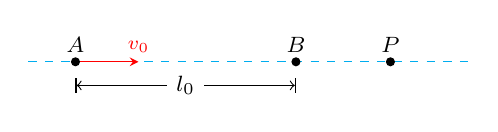
\begin{tikzpicture}
	\draw[dashed,cyan] (-.6,0)--(5,0);
	\draw[-stealth,red] (0,0)--(.8,0)node[above]{\scriptsize \(v_0\)};
	\foreach \x/\c in{0/A,2.8/B,4/P}
		\draw[fill=black] (\x,0)node[above]{\footnotesize \(\c\)} circle(.05);
	\draw[|<->|,thin] (0,-.3)--node[fill=white]{\footnotesize \(l_0\)}(2.8,-.3);	
\end{tikzpicture}
\begin{answer}
	(1)\(\frac{1}{5}v_0\)\qquad (2) \(\frac{v_0t_1}{5} - \frac{2}{11}l_0\)\qquad (3) \(\frac{2l_0}{v_0}\)
\end{answer}